\section{Multiprocessori e MultiComputer}
Il modo forse più diretto per implementare il parallelismo è quello di aggiungere più processori, creando un \textbf{multiprocessore}.

Se essi condividono la stessa memoria essi possono essere trattati come un unico processore e sono un esempio di un sistema \textit{strongly coupled}.

\begin{figure}[H]
    \centering
    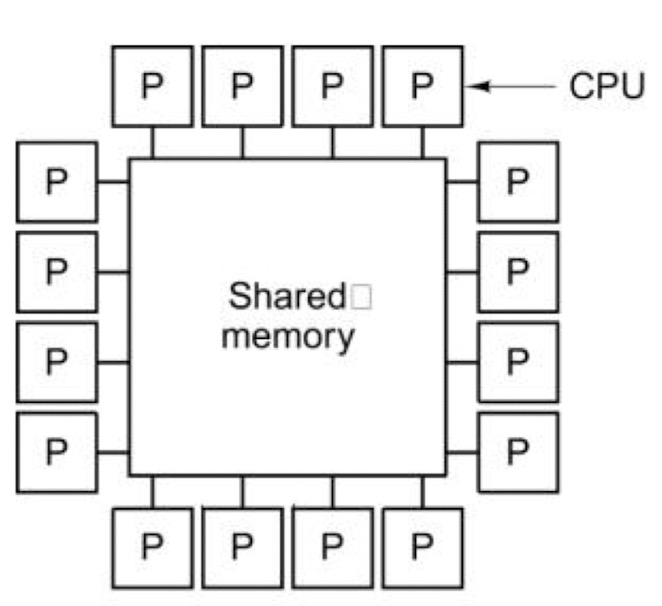
\includegraphics[width=0.28\linewidth]{assets/multiprocessore.jpg}
\end{figure}

Per inserire una potenza di calcolo ancora maggiore è necessario unire due o più multiprocessori in un \textbf{multicomputer}.

In questo caso risulta essere più complessa la programmazione, in quanto i sistemi sono \textit{loosely coupled} ed è necessario tenere conto degli overhead dello scambio di informazioni, ma a livello hardware sono molto più semplici da costruire a parità di core.

\begin{figure}[H]
    \centering
    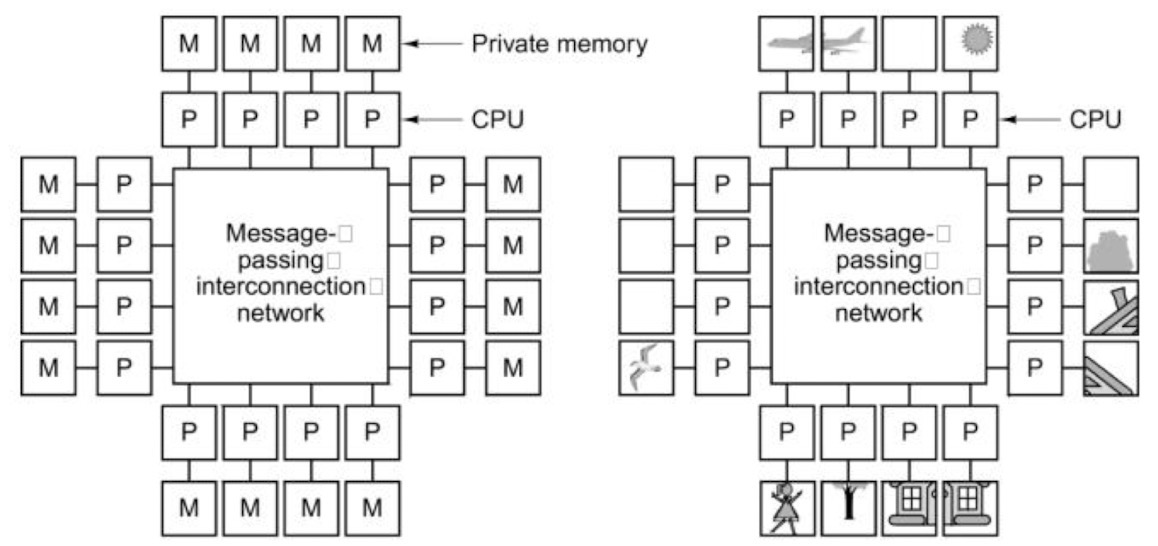
\includegraphics[width=0.62\linewidth]{assets/multicomputer.png}
\end{figure}

\begin{note}
    Quando due SoC sono connessi con una connessione con larghezza di banda sufficiente essi possono essere trattati come un unico chip. Ad esempio la serie Ultra dei chip Apple Silicon ha una connessione "DeepFusion" a 2.5 TB/s a bassa latenza.
\end{note}

\subsection{Topologia delle Connessioni}

In un sistema multicomputer la \textbf{topologia} delle connessioni tra i vari computer diventa di centrale importanza, si cercano le migliori prestazioni riducendo la quantità di connessioni necessarie.

\begin{figure}[H]
    \centering
    \begin{minipage}{0.45\textwidth}
        \subsubsection{Grado o fanout}
        Il numero di connessioni che passano per un nodo, un grado maggiore indica maggiori tolleranze a possibili interruzioni di rete.
    \end{minipage}
    \hfill
    \begin{minipage}{0.45\textwidth}
        \begin{figure}[H]
            \centering
            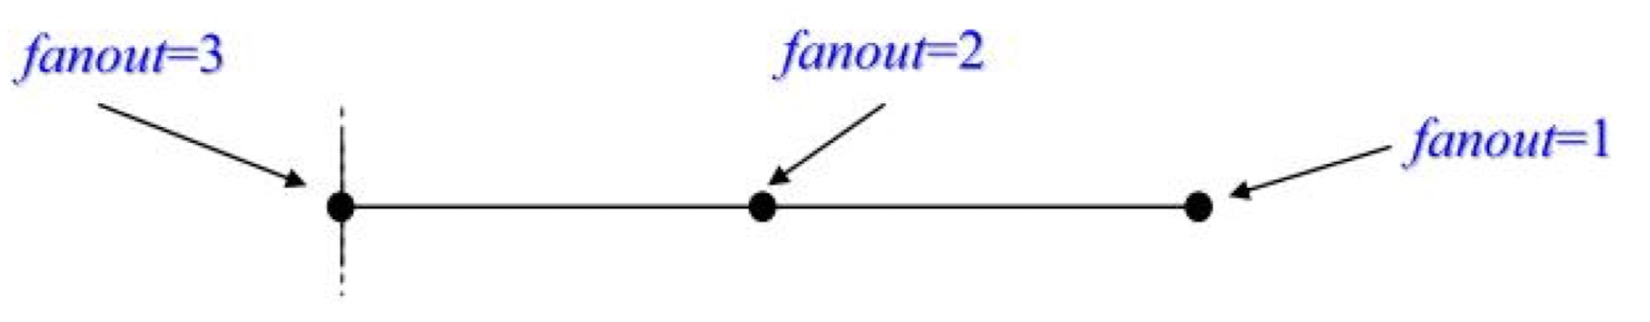
\includegraphics[width=1\linewidth]{assets/fanout.jpg}
        \end{figure}
    \end{minipage}
\end{figure}

\begin{figure}[H]
    \centering
    \begin{minipage}{0.45\textwidth}
        \subsubsection{Diametro}
        Il numero massimo di passaggi tra un nodo e un'altro in una rete, dà informazioni sul tempo di comunicazione nel caso peggiore.
    \end{minipage}
    \hfill
    \begin{minipage}{0.45\textwidth}
        \begin{figure}[H]
            \centering
            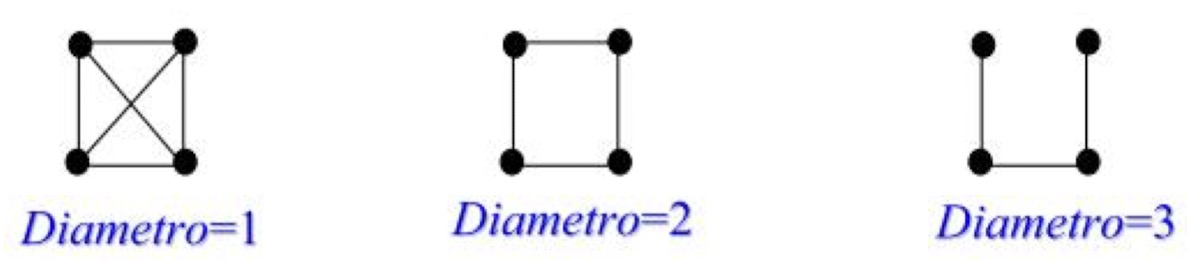
\includegraphics[width=1\linewidth]{assets/diametro.jpg}
        \end{figure}
    \end{minipage}
\end{figure}

\begin{figure}[H]
    \centering
    \begin{minipage}{0.45\textwidth}
        \subsubsection{Dimensionalità}
        Numero di assi che devono essere percorsi per arrivare dal un nodo ad un'altro (caso massimo).
    \end{minipage}
    \hfill
    \begin{minipage}{0.45\textwidth}
        \begin{figure}[H]
            \centering
            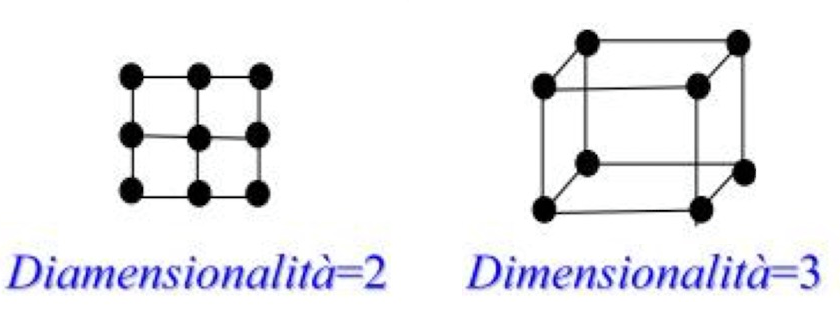
\includegraphics[width=0.65\linewidth]{assets/dimensionalita.png}
        \end{figure}
    \end{minipage}
\end{figure}

\begin{figure}[H]
    \centering
    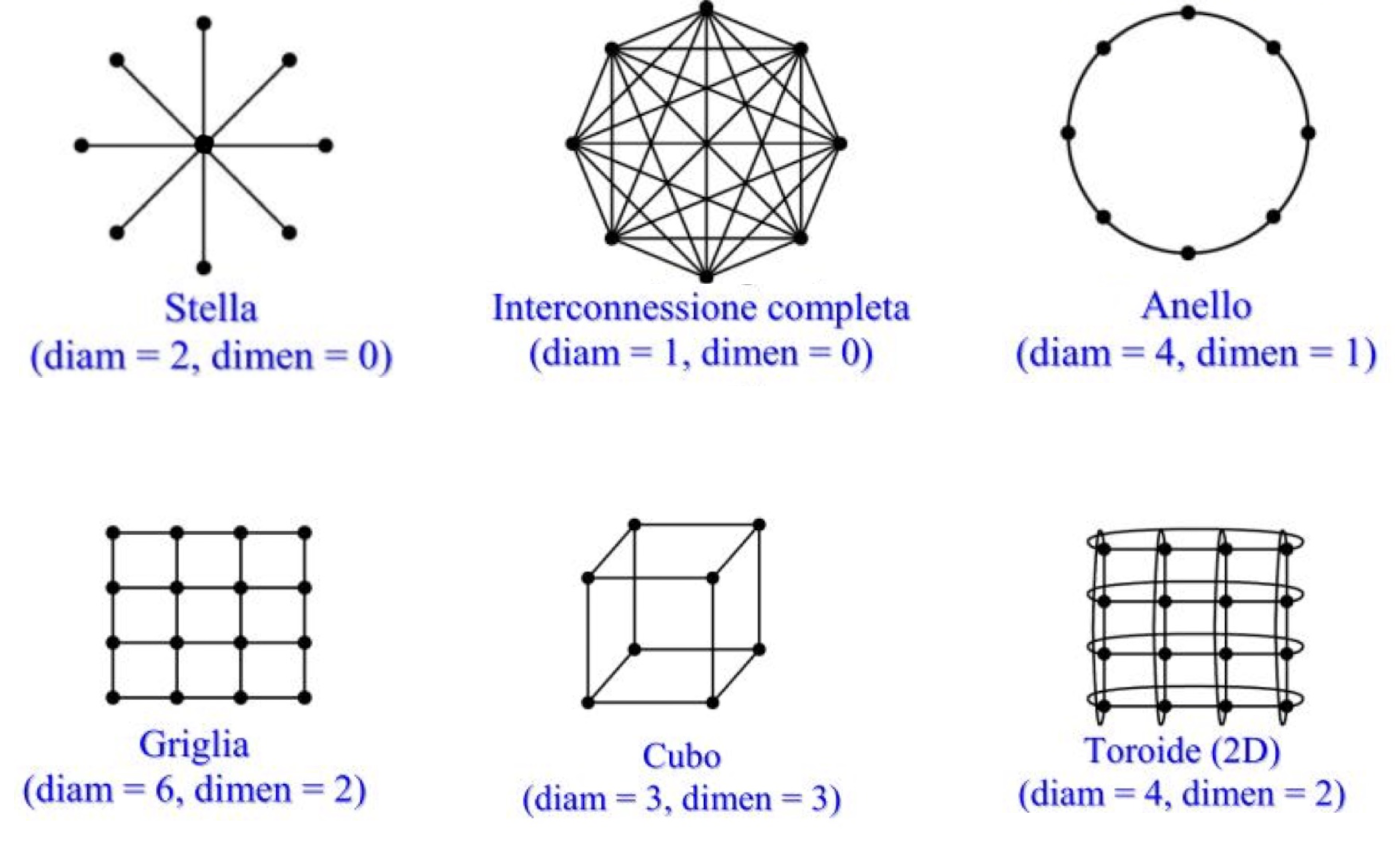
\includegraphics[width=0.5\linewidth]{assets/connessioni.png}
    \caption{Esempi di connessioni}
\end{figure}

\begin{note}
    Nei supercomputer nella maggior parte dei casi si opta per una connessione a toroide 3D, quindi ha dimensione 3, che porta un buon compromesso tra diametro e numero di connessioni.

    \begin{figure}[H]
        \centering
        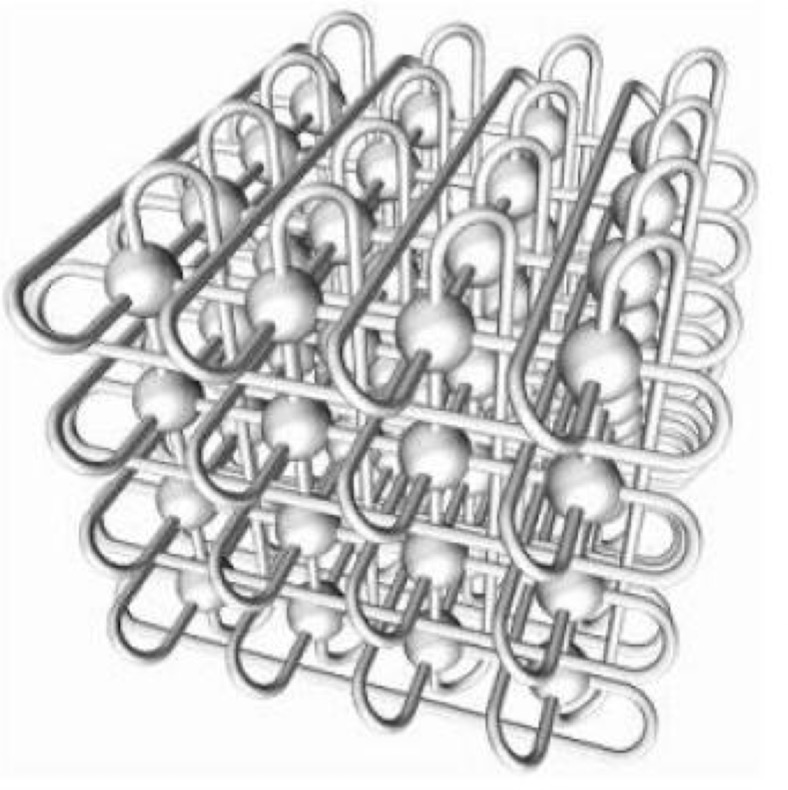
\includegraphics[width=0.3\linewidth]{assets/toroide3d.jpg}
        \caption{Toroide(3D)}
    \end{figure}
\end{note}

\subsection{Prestazioni}
Vogliamo calcolare quanto aumentano le prestazioni se applichiamo $n$ CPU allo stesso problema.

Ovviamente è impossibile ottenere un aumento delle prestazioni pari a $n$.

\spacer
\begin{sitemize}
    \item Esistono parti dei programmi \textbf{intrinsecamente sequenziali}.
    \item La \textbf{comunicazione}, per quanto efficiente, comporta dell'overhead.
    \item Gli \textbf{algoritmi paralleli} sono spesso sub-ottimi rispetto a quelli sequenziali.
\end{sitemize}

$$T_{es, parallelo} = f\cdot T_{es, sequenziale} + \frac{(1-f)\cdot T_{es, sequenziale}}{n}$$

dove $f$ è la frazione di codice sequenziale sul totale.

\subsubsection{Prestazioni e Connessioni}
Aumentare il numero di CPU spesso non è sufficiente per incrementare le prestazioni. È necessario avere un'architettura \textbf{scalabile}.

Delle buone struttura di topologia delle connessioni sono a griglia e a cubo, mentre quella ottimale è l'ipercubo, in quanto il diametro aumenta logaritmicamente rispetto al numero dei processori.

\subsection{Tassonomia o Classificazione dei sistemi}
Quella più utilizzata è quella ideata da Flynn nel 1972 che si basa sulla grandezza delle sequenze di numeri e di dati.

\begin{center}
    \begin{tabular}{ | c | m{2cm} | m{2cm} | c | }
        \hline
        Nome & \raggedright Sequenze di istruzioni & \raggedright Sequenze di dati & Esempi                         \\
        \hline \hline
        SISD & 1                                   & 1                             & Macchina di Von Neumann        \\
        SIMD & 1                                   & Molte                         & Computer Vettoriali            \\
        MISD & Molte                               & 1                             & Solo teoriche                  \\
        MIMD & Molte                               & Molte                         & Multiprocessori, Multicomputer \\
        \hline
    \end{tabular}
\end{center}

\subsection{Implementazioni}

\subsubsection{NUMA}
Spesso il fattore limitante al numero di processori che è possibile aggiungere ad un sistema è la dimensione del bus che porta alla memoria principale.

\spacer
Nell'architettura NUMA si fornisce ad ogni processore una \textbf{memoria locale} a cui può accedere con un suo bus separato.

Inoltre tutti i processori condividono gli stessi indirizzi fisici, quindi la comunicazione tra processori può avvenire facilmente tramite una connessione diretta.

\spacer

Questo rende molto più semplice scalare i sistemi e accelera i tempi di accesso tra il processore e la sua memoria, tuttavia l'accesso alla memoria di un'altro processore è molto rallentato.

\begin{figure}[H]
    \centering
    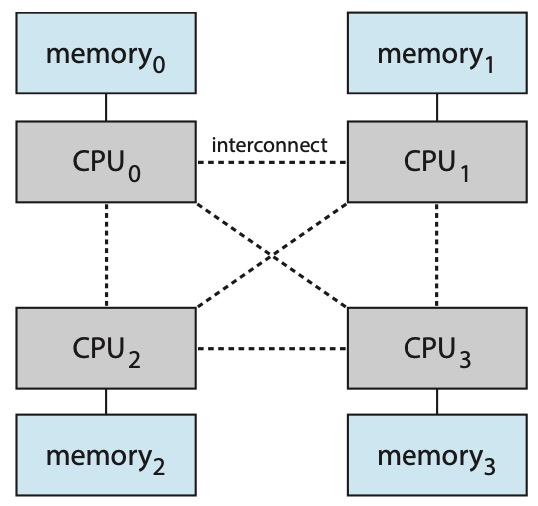
\includegraphics[width=0.3\linewidth]{assets/NUMA.jpg}
    \caption{Visualizzazione sistema NUMA}
\end{figure}

\subsubsection{Cluster}
In modo simile a quanto possiamo fare per più processori possiamo collegare due o più calcolatori completi. I quali possono condividere una memoria secondaria comune.
Questi sistemi sono debolmente accoppiati, quindi non tutte le operazioni possono sfruttare la completa potenza di calcolo.

Anche in questo caso è possibile creare cluster \textbf{asimmetrici} e \textbf{simmetrici}, i primi possiedono un nodo che ha l'unica funzione di gestire gli altri rimanendo in uno stato di attesa attiva, mentre nei secondi tutti i nodi eseguono le applicazioni e si controllano reciprocamente.

\begin{figure}[H]
    \centering
    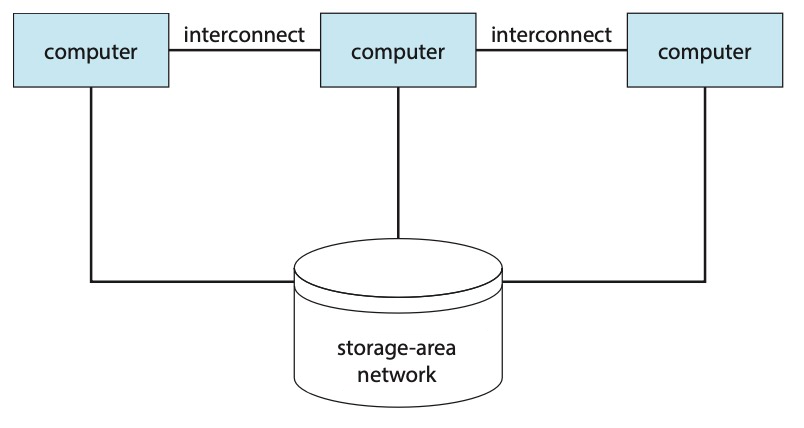
\includegraphics[width=0.5\linewidth]{assets/cluster.png}
    \caption{Cluster}
\end{figure}

\begin{note}
    Questo risulta essere particolarmente utile nel caso di sistemi che devono essere sempre operativi, anche nel caso di un malfunzionamento di uno dei computer il servizio non viene interrotto.

    \spacer
    I Cluster vengono utilizzati anche nell'\textit{High performance computing}, ma le applicazioni devono essere scritte appositamente per poter sfruttare tutte le prestazioni messe a disposizione dal cluster.
\end{note}

\subsection{Coprocessori}
Un coprocessore è un processore \textbf{indipendente} che esegue compiti specializzati sotto il controllo del processore principale.

\spacer
\begin{sitemize}
    \item \textbf{Coprocessori di rete:} Specializzati per gestire ad alta velocità i pacchetti di rete.
    \item \textbf{Crittoprocessori:} Consentono di cifrare/decifrare velocemente flussi di dati.
    \item \textbf{Graphical Processing Unit (GPU):} Consente di processare una gran quantità di dati video e grafica 3D. Una singola GPU può contenere fino a qualche migliaio di core grafici.
    \spacer
    Le GP-GPU, \textit{general purpose GPU} grazie a linguaggi di programmazione quali CUDA e OpenCL possono essere facilmente utilizzate per operazioni floating point, rendendole così di grande importanza nell'high performance computing.
    \spacer
    Per ottenere questo tipo di schede grafiche è stato necessario convertire i core per renderli compatibili alle specifiche IEEE per l'aritmetica a singola e doppia precisione. Inoltre è stato necessario fornire accesso in lettura e scrittura alla memoria principale.
    \item \textbf{Tensor Processing Unit (TPU):} Un coprocessore dedicato alle reti neurali per il \textit{deep learning}.
    \item \textbf{Field Programmable Gate Array (FPGA):} È un dispositivo che permette di implementare algoritmi in hardware, tramite software.

    Presenta una serie di blocchi logici configurabili e sono ideali per lo sviluppo e per dei prototipi rapidi.
\end{sitemize}
